\documentclass{article}
\usepackage{lipsum}
% Language setting
% Replace `english' with e.g. `spanish' to change the document language
\usepackage[english]{babel}
% Set page size and margins
% Replace `letterpaper' with `a4paper' for UK/EU standard size
\usepackage[letterpaper,top=2cm,bottom=2cm,left=3cm,right=3cm,marginparwidth=1.75cm]{geometry}

% Useful packages
\usepackage{amsmath}
\usepackage{graphicx}
\usepackage{subcaption}
\usepackage{wrapfig}
\usepackage{pdfpages}
\usepackage{lipsum}
% \usepackage[colorlinks=true, allcolors=blue]{hyperref}

\usepackage{color}   %May be necessary if you want to color links
\usepackage{hyperref}
\hypersetup{
    colorlinks=true, %set true if you want colored links
    linktoc=all, 
    linkcolor=blue,
}
\usepackage{cleveref}
% More defined colors
\usepackage[dvipsnames]{xcolor}

% Required package
\usepackage{tikz}
\usetikzlibrary{positioning}

\title{Foundations of Deep Learning}
\author{Geralyn Chong}
\begin{document}
\maketitle
\tableofcontents

\section{Token classification}
Token classification transforms unstructed into structured data. For example, Name-Entity recognition is a kind of token classification is used to recognize certain entities in a text by labeling segments of text:\\ 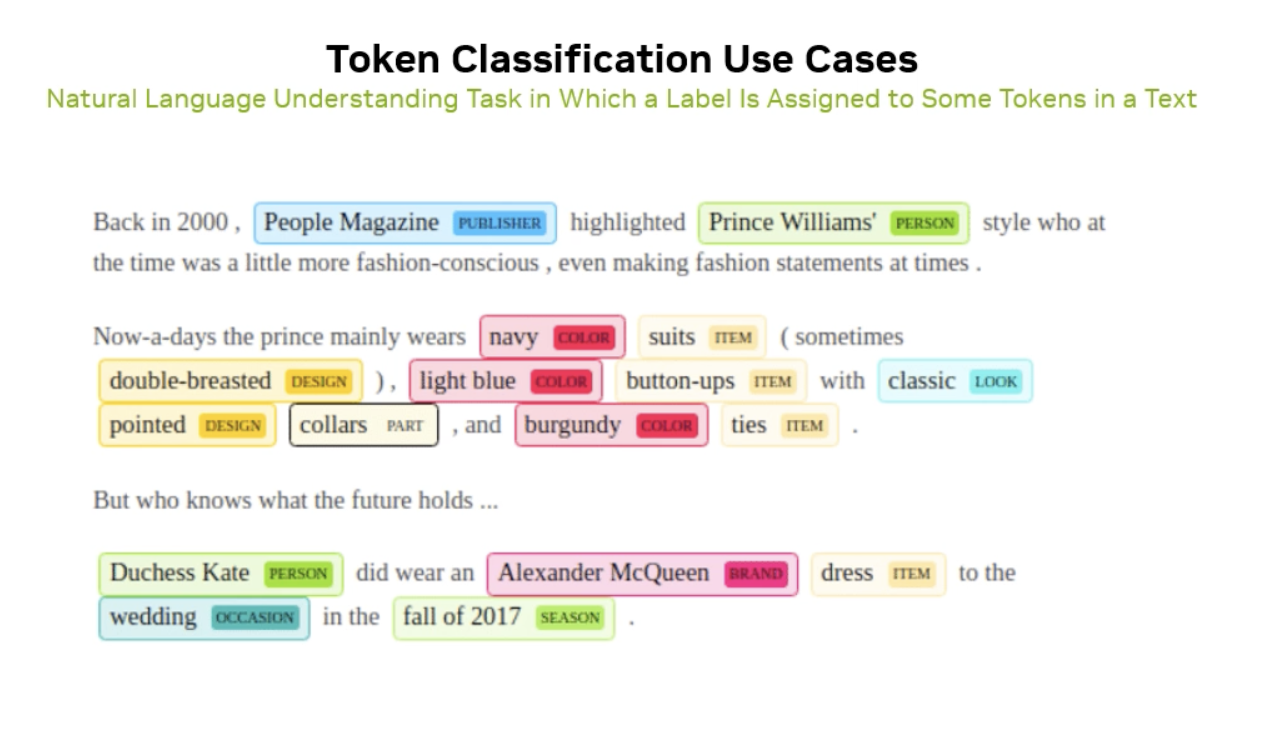
\includegraphics[width=0.9\textwidth]{../images/npr.png}

We can also identify custom entities for specific task use cases. The example below indicates a type of tokenization architecture that includes BERT (Bidirectional Encoder Representations for Transformers) and a classification layer. In this case, we want to assign labels to the output from BERT. \href{https://huggingface.co/docs/transformers/en/tasks/token_classification}{A hugging face tutorial that is adjacent to this concept. }\\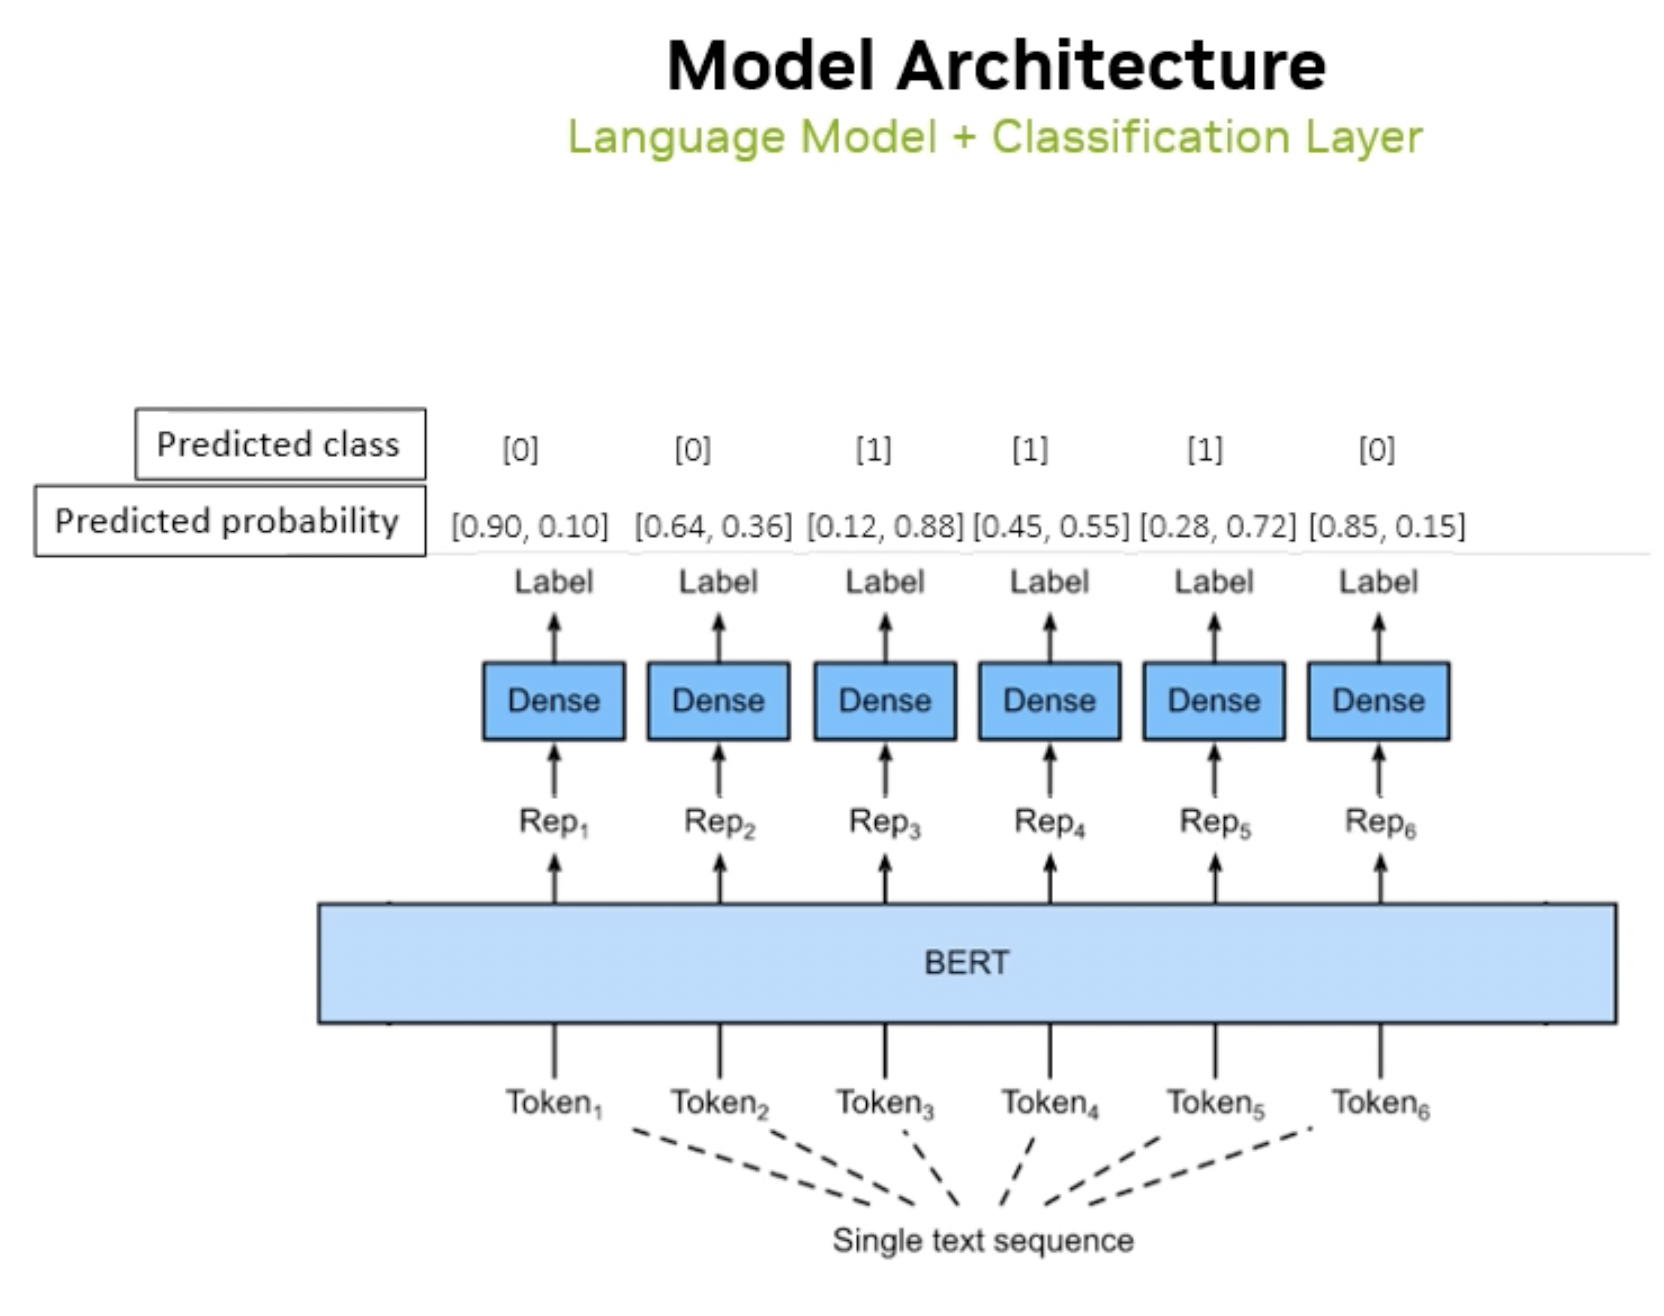
\includegraphics[width=0.9\textwidth]{../images/bertToken.png}

\subsection{NeMo: A toolkit for Conversational AI}
NeMo framework provides NLP capabilities along with Automatic Speech recognition (ARS), and Text-to-Speech (TTS).\\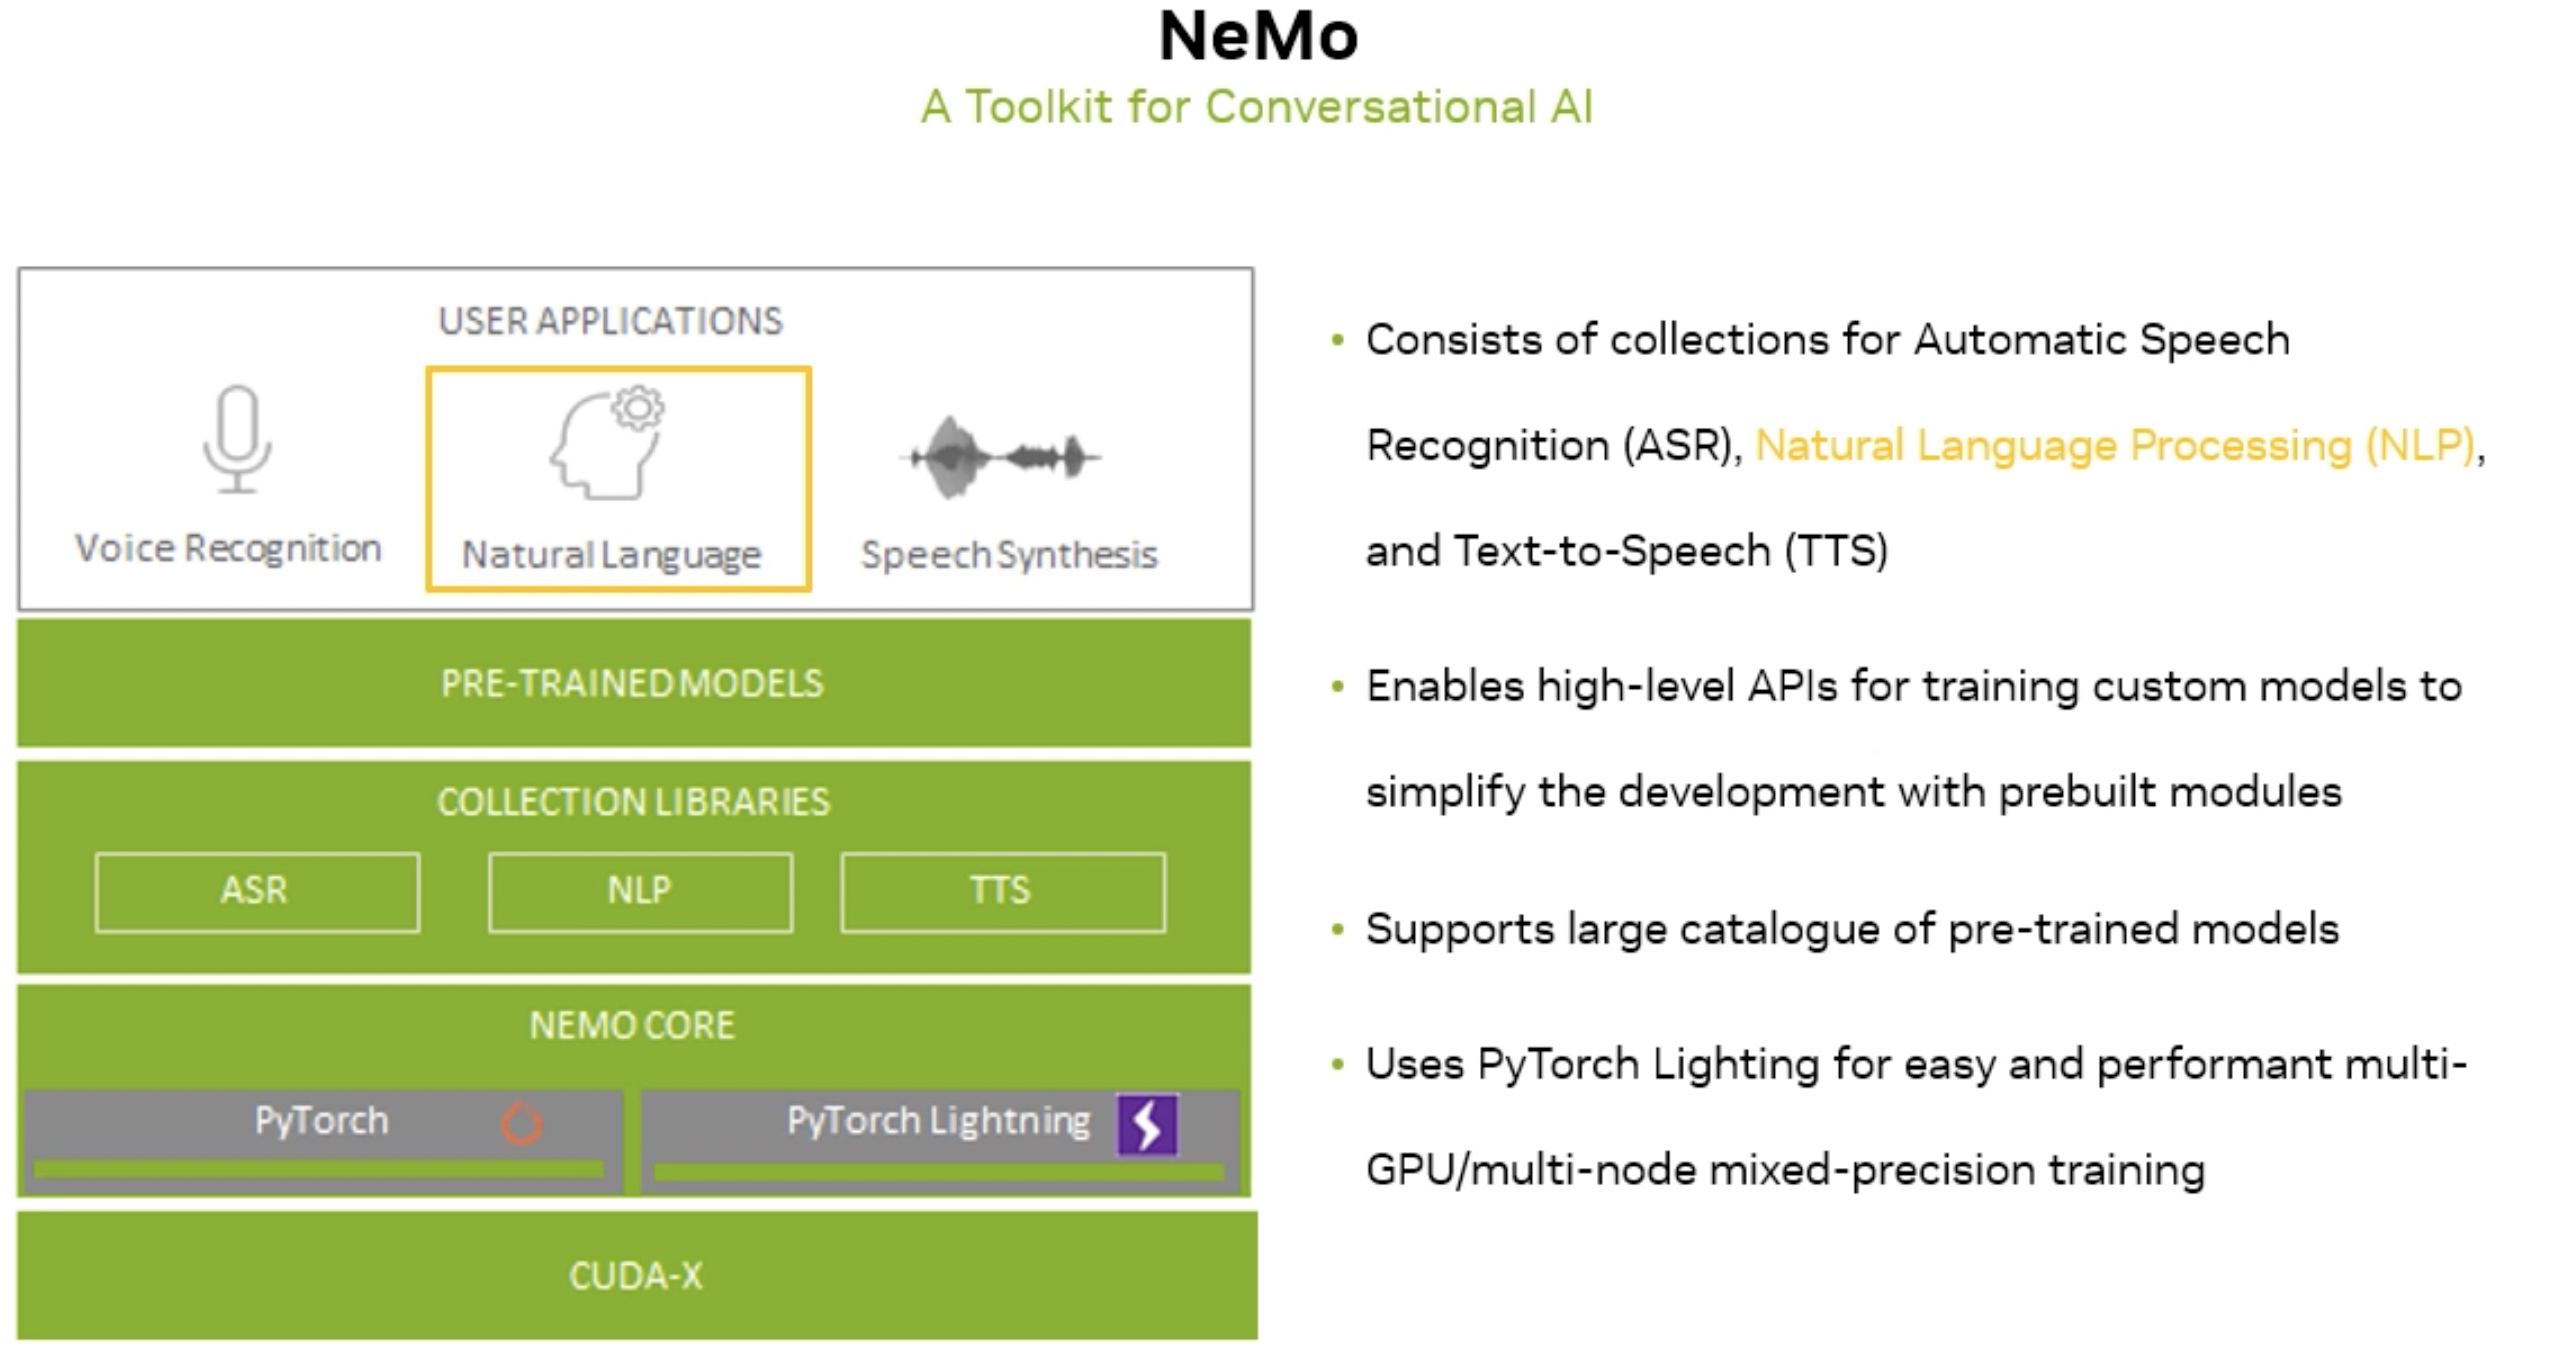
\includegraphics[width=0.9\textwidth]{../images/nemoStructure.png} \\\href{https://docs.nvidia.com/nemo-framework/user-guide/latest/overview.html}{Here} is the official documentation for Nvidia's NeMo framework. 

Using this pre-built component for recognition of token sections, we can perform tokenization, position embedding, padding, attention masking, and more. This allows us to build custom tokenization models.

\subsection{Lab 1: Name-Entity Recognition Practice}
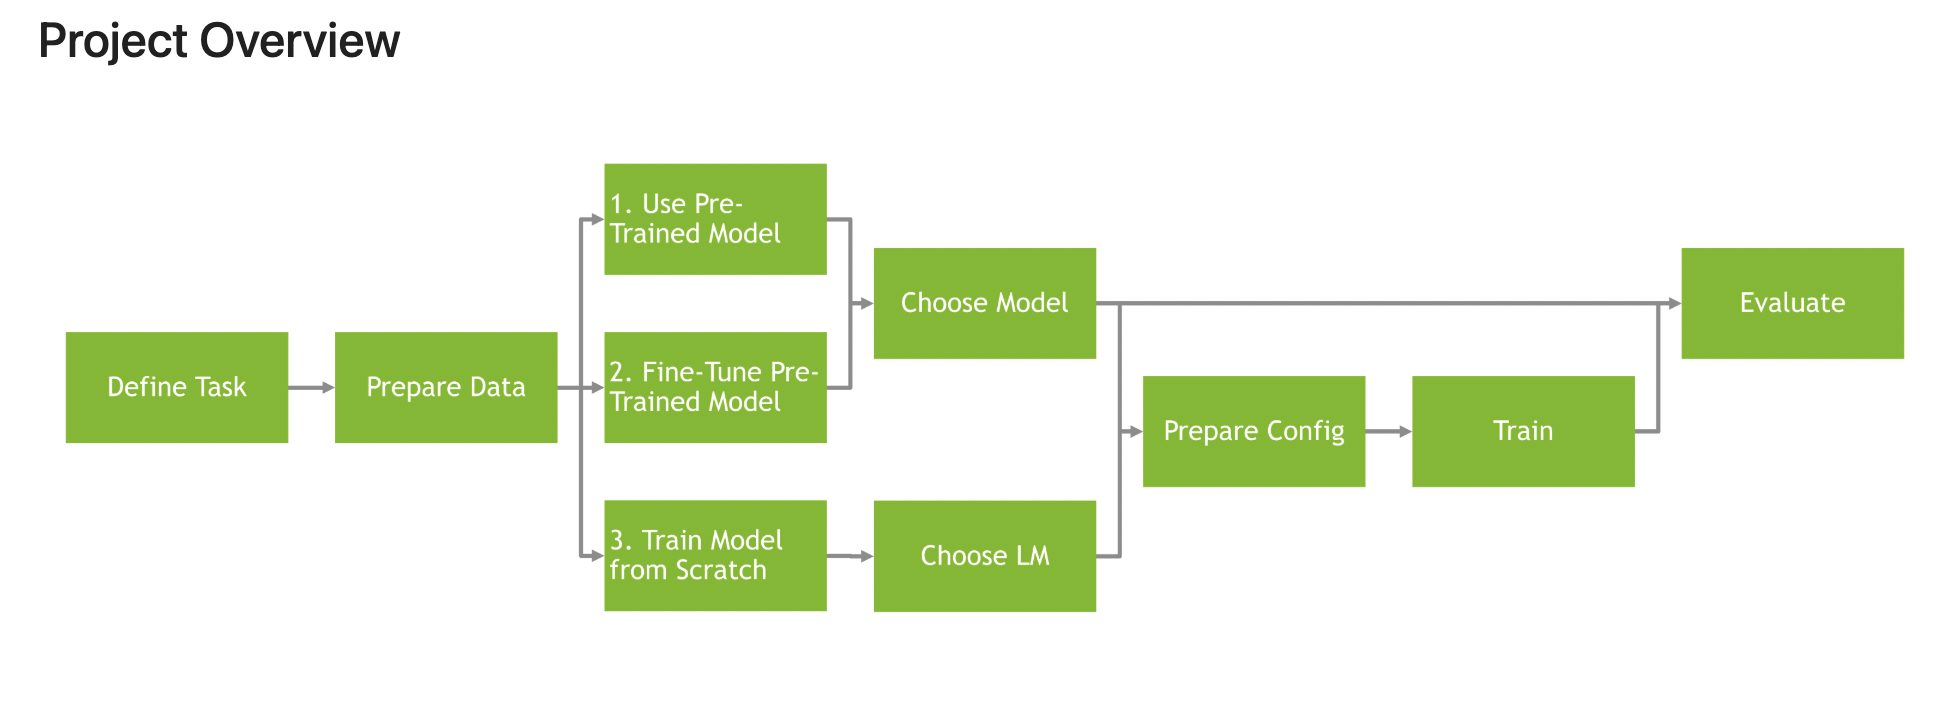
\includegraphics[width=\textwidth]{../images/lab1NER_overview.png}\\
\subsubsection{Lab Overview and Steps}
\begin{enumerate}
    \item Dataset choice
    \item NeMo Architecture Requirements
    \item Using a Pre-trained model
\end{enumerate}

\noindent\begin{Large}\textit{Dataset Choice}\end{Large}\vspace{10pt}\\
\indent The lab utilizes the Groningen Meaning Bank (GMB) which represents a large set of labelled classes including Geographical entity (LOC), Organization (ORG), Person (PER), Geopolitical Entity (GPE), Time indicator (TIME), Artifact (ART), Event (EVE), and Natural Phenomenon (NAT). Note: The dataset is not $100\%$ human-labelled so the dataset is not considered entirely ground-truth. The data is also labelled using IOB format where each annotation has a prefix of \textbf{I}, \textbf{O}, and \textbf{B}.\vspace{15pt}\\ 

\noindent\begin{Large}\textit{NeMo Architecture Requirements}\end{Large}\vspace{10pt}\\
In order to feed in our "ground-truth" labels for our pre-built module like BERT to learn the specific labels for each category that we would like to recognize, we need to feed in a \verb|text.txt| and a \verb|labels.txt| file for our entities and their corresponding labels. 

This step assumes that the preprocessing of our label data is complete. Suppose that you have raw data, NeMo is compatible with Datasaur. \href{https://www.youtube.com/watch?v=I9WVmnnSciE}{Here is a tutorial for it.} The NeMo model also includes built-in methods that take advantage of these capabilities: \verb|TokenClassificationModel.add_predictions()| and \verb|TokenClassificationModel.evaluate_from_file()| which are inherited from the \verb|NLPModel| \vspace{15pt}\\ 

% \noindent\begin{Large}\textit{Using Pre-trained model}\end{Large}\vspace{10pt}\\



\end{document}